%%%%%%%%%%%%%%%%%%%%%%%%%%%%%%%%%%%%%%%%%
% Journal Article
% LaTeX Template
% Version 2.0 (February 7, 2023)
%
% This template originates from:
% https://www.LaTeXTemplates.com
%
% Author:
% Vel (vel@latextemplates.com)
%
% License:
% CC BY-NC-SA 4.0 (https://creativecommons.org/licenses/by-nc-sa/4.0/)
%
% NOTE: The bibliography needs to be compiled using the biber engine.
%
%%%%%%%%%%%%%%%%%%%%%%%%%%%%%%%%%%%%%%%%%

%----------------------------------------------------------------------------------------
%	PACKAGES AND OTHER DOCUMENT CONFIGURATIONS
%----------------------------------------------------------------------------------------

\documentclass[
	a4paper, % Paper size, use either a4paper or letterpaper
	10pt, % Default font size, can also use 11pt or 12pt, although this is not recommended
	unnumberedsections, % Comment to enable section numbering
	twoside, % Two side traditional mode where headers and footers change between odd and even pages, comment this option to make them fixed
]{LTJournalArticle}

\addbibresource{ref.bib} % BibLaTeX bibliography file


\setcounter{page}{1} % The page number of the first page, set this to a higher number if the article is to be part of an issue or larger work

\usepackage{url}

\usepackage{graphicx}             % For including images
\usepackage{subfigure}
\usepackage{adjustbox}            % For scaling and packing
\usepackage{subcaption}           % For subfigures
\usepackage{xcolor}         % For color names
\usepackage{hyperref}       % For hyperlinks and colored citations

%%%%

\usepackage{amssymb,amsthm,amsmath}
\usepackage{multirow,epsfig, times,multicol}
\usepackage[mathscr]{eucal}
\usepackage{amsfonts}
\usepackage{wrapfig}
\usepackage{amssymb}

\usepackage{ifthen}


\usepackage{titlesec}

\titlespacing*{\section} % Adjusts section spacing
  {0pt}   % Left indent (usually 0pt for no indent)
  {2pt}  % Space above the section title
  {2pt}   % Space below the section title

\titlespacing*{\subsection}
  {0pt}{2pt}{2pt}


%%%%

% Set colors for links and citations
\hypersetup{
    colorlinks=true,        % Enable colored links
    linkcolor=orange,        % Set link color (e.g., section refs)
    citecolor=blue,         % Set citation color
    urlcolor=cyan           % Set URL color
}



\usepackage{listings}


\lstset{
    basicstyle=\ttfamily, % Use typewriter font
    keywordstyle=\color{blue}, % Keywords in blue
    commentstyle=\color{green!50!black}, % Comments in green
    stringstyle=\color{red}, % Strings in red
    backgroundcolor=\color{gray!10}, % Light gray background
    numbers=left, % Line numbers on the left
    numberstyle=\tiny\color{gray}, % Style for line numbers
    frame=single, % Single frame around code
    tabsize=2, % Set tab size
}

\usepackage{enumitem} % Recommended package for list customization

\setlist[itemize]{topsep=1pt, itemsep=0pt, parsep=1pt, partopsep=0pt}
\setlist[enumerate]{topsep=1pt, itemsep=0pt, parsep=1pt, partopsep=0pt}
\setlength{\topsep}{0pt}     % Space before and after the environment
\setlength{\partopsep}{0pt}   % Extra space added before if needed
\setlength{\parskip}{0pt}     % Space between paragraphs inside verbatim (optional)
\graphicspath{{figures/}}


%----------------------------------------------------------------------------------------
%	TITLE SECTION
%----------------------------------------------------------------------------------------

\title{CP 217: Project 2 Report} % Article title, use manual lines breaks (\\) to beautify the layout

% Authors are listed in a comma-separated list with superscript numbers indicating affiliations
% \thanks{} is used for any text that should be placed in a footnote on the first page, such as the corresponding author's email, journal acceptance dates, a copyright/license notice, keywords, etc
\author{%
	Subhasis Biswas\thanks{22571, CDS MTech 2nd Year},  Pradhumn Sharma\thanks{22559, CDS MTech 2nd Year} and Bhookya Raju\thanks{25076, MTech Mobility Engg \& Mech Dept}
}

% Affiliations are output in the \date{} command


%----------------------------------------------------------------------------------------

\begin{document}

% \onecolumn
% \maketitle % Output the title section

\begin{center}
  \textbf{\Large CP 217: Project 2 Report} \\[1em]
  \textbf{Team: Data Diviners} \\[2em]
\end{center}
\vspace{-8pt}
\textbf{Subhasis Biswas} \> (22571, CDS MTech 2nd Year) \\
\textbf{Pradhumn Sharma} \> (22559, CDS MTech 2nd Year) \\
\textbf{Bhookya Raju} \> (25076, MTech Mobility Engg \& Mech Dept) \\


% \thispagestyle{empty}
% \mbox{} % Empty box to force the page

% \newpage
\vspace{-8pt}

\section{Part A}



\subsection{A.1}

In this section we refer to the defined metrics as $M1$, $M2$ and $M3$.
\begin{itemize}
    \item \textbf{M1}: Geographic Proximity
    \item \textbf{M2}: Service Availability
    \item \textbf{M3}: Population Age Distribution
\end{itemize}

\subsubsection{Metric Specifications}\leavevmode


Here we'll be going through how the similarity metrics were defined and the related information.

\textbf{M1}: Used $Location$ feature from the excel sheets to approximate the location relative to the \textit{Melbourne General Post Office (GPO)}. The feature-value was parsed as: \newline
\textit{Xkm Y of Melbourne} $\rightarrow (X, Y) \rightarrow (X, compass\ bearing)$, with $Y \in \{\text{N}, \text{NNE}, \text{NE}, \text{ENE}, \dots,\text{NNW}\}$ and the corresponding bearings being in $\{0, 22.5, 45, 67.5,\dots, 337.5\}$.

Now, max distance of any suburb from our origin $O$ (Melbourne GPO) is 68km. So, maximum pairwise distance that can be is $2\times 68=136$ km. The curvature of the Earth causes a drop of around $1.45km$ [\href{https://earthcurvature.com/}{Calculator}] across this distance. As this is quite small, it's ignored and the entire region is treated as flat. We then convert $Polar$ to $Cartesian$ using the formula 

$(x, y) = \big(r\sin\left(\frac{\pi\theta}{180}\right), r\cos\left(\frac{\pi\theta}{180}\right)\big)$ [$y$ axis aligns with $0^\circ$, so $\sin$ and $\cos$ are swapped]. The goal is to check for physical proximity of the suburbs, using the $L^2$ norm.

\textbf{M2}: Each feature under the $Services$ catgory is considered and min-max scaled. Afterwards, mean was taken across the scaled feature-values under the Services category suburb by suburb, which is named as the $Services \ Score$ for that suburb. Similarity between suburbs from this perspective is defined as the absolute difference between the corresponding services' score. The aim is to quantify how well-equipped a suburb is in terms of the said facilities and to check for similar amount of services provided in other suburbs.

\textbf{M3}: The \textit{2012 population} category was chosen and only the feature names with $\%$ were chosen, for example

$\{ \textit{2012 ERP age 0-4\%}, \textit{2012 ERP age 5-9\%}, \dots\}$. The feature values are then converted to probability distributions, with each row summing up to 1 for each suburb (verified). For quantifying similarity between two locations we consider the \href{https://en.wikipedia.org/wiki/Jensen%E2%80%93Shannon_divergence}{Jensen Shannon Divergence}(JSD) between the two population distributions. This distance metric was chosen as we're essentially dealing with pmf's and because JSD is symmetric. The aim of this metric is to measure the similarity between the 2012 (latest) population distributions between two locations.



\subsection{A.2}

We are using the following module for computing the multidimensional scaling onto 2D.
\begin{verbatim}
    from sklearn.manifold import MDS
\end{verbatim}

We'll be using \href{https://en.wikipedia.org/wiki/Procrustes_analysis}{Procrustes Disparity} for measuring the alignment between two distance metrics, the comparisons might be of the sort: \textit{Metric in original space vs Metric in 2D} or \textit{Metric A vs Metric B} etc. The closer the value of the disparity is to 0 the better. For MDS, we'll also note the \href{https://imaging.mrc-cbu.cam.ac.uk/statswiki/FAQ/mds/stress#:~:text=The%20measure%20of%20goodness%20of,or%20more%20estimated%20stimuli%20dimensions}{stress of the MDS} and the correlation between the original pairwise distances and distances in the 2D projected space. The values of the MDS quality metrics are written within the plots.

\textbf{M1}: The suburb locations are already on the 2D map, thus we do not require MDS.  \hyperref[sub@fig:jd_suburb_dist]{Figure~\ref{fig:jd_suburb_dist}} \hyperref[sub@fig:scatter_suburb]{Figure~\ref{fig:scatter_suburb}}

\textbf{M2}: 2D projected profile: \hyperref[sub@fig:mds_services]{Figure~\ref{fig:mds_services}}

\textbf{M3}: 2D projected profile: \hyperref[sub@fig:mds_population]{Figure~\ref{fig:mds_population}}




\subsubsection{Findings}

While doing MDS, for the service score metric, we're essentially dealing with scalar outputs, and trying to put them in 2D. Thus the distance has been well preserved between the original and the 2D space as indicated by the low stress and disparity as well as high correlation. This was expected.

However, for JSD based population distribution similarity, the high amount of stress indicates poor projection onto the 2D. Although it's not exactly a surprise but still that's quite a high amount. Despite of that, the disparity is still low and correlation is high. 


To check which suburbs remain unchanged between these two metrics \textit{M2} and \textit{M3} (we deal with geographic proximity later on) we do a \href{https://en.wikipedia.org/wiki/Spectral_clustering}{spectral clustering} with the exact same similarity matrices arising out of the original computation. Then we use a Gaussian Kernel with $\sigma=1$. We check for the 'elbow' in the (sorted in descending order) eigenvalue plots for both M2 and M3 for the affinity matrices and decide upon the number of clusters required. We settle on $k=3$. The agreement between the two clusterings:

$ARI=0.024, NMI=0.133$;  \hyperref[sub@fig:spectral_clustering]{Figure~\ref{fig:spectral_clustering}}


\subsection{A.3}


The issue with geospatial data analysis is that the observations of the neighbouring places are not independent, thus many of the ML algorithms that assume independence of the samples cannot be used here directly. Here, in order to address the \href{https://www.sciencedirect.com/topics/mathematics/spatial-autocorrelation}{Spatial Autocorrelation} we use \href{https://en.wikipedia.org/wiki/Moran%27s_I}{Moran's I} (both Global and Local, with permutations set to 9999, random seed = 42) for testing the influence of the geographic proximity. More formally, for Moran's I hypothesis test we set the null hypothesis $H_0$ as:

$H_0:$ \textit{There is no spatial autocorrelation between the observations}

with significance level set to $\alpha =0.05$. Weight matrix was constructed using KNN with $k=8$ (\href{https://pro.arcgis.com/en/pro-app/latest/tool-reference/spatial-statistics/spatial-autocorrelation.htm}{Recommendation}) due to the varying spatial density of the suburbs.

We then run Moran's I test (without reducing power of the test) for each individual features across all the suburbs considered for the metrics of M2 and M3 and note the $p-value$ (Note: This test takes in only one feature at a time). If $p<\alpha$ for a feature $F$, we conclude that $F$ has significant spatial autocorrelation, i.e. geographic proximity has significant effect on $F$.

\subsubsection{M2}\leavevmode

Moran's I for Services Score: -0.00848

Moran's I p-value: 0.31300

\% of significant features (out of the all features for M2): 21\%

\% of feature-value of significant features: 15.25\%

(Out of the total values across all the suburbs and all the features. This works since all the values are non-negative.)

Procrustes Disparity between suburb $L^2$ distances and M2: 0.868

\hyperref[fig:moran_part_A]{Figure~\ref{fig:moran_part_A} Moran Statistics plot with p-values}


\subsubsection{M3}\leavevmode

\% of significant features (out of the all features for M3): 50\%

\% of feature-value of significant features: 77.90\%

Procrustes Disparity between suburb $L^2$ distances and M3: 0.747

\hyperref[fig:moran_part_A]{Figure~\ref{fig:moran_part_A} Moran Statistics plot with p-values}


\subsubsection{Conclusion}\leavevmode

The data partially supports the hypothesis, and depends on the perspective and the metric chosen. Some features being considered under the same metric may be significantly affected by physical proximity, while some may not be. Thus, we decided to consider the weight contributed by the feature values. Unsurprisingly, due to larger weight of M3 features as compared to M2, the disparity between the physical distance based proximity and M3 is much lower than that of disparity between M2 and physical distance.

\pagebreak

\section{Part B}

\subsection{B1.}

\subsubsection{Analysis focused on Hospitals}

We collected the actual locations of the hospitals from Google Maps and plotted them, in order to get an approximate idea of their positions. <Figure>

To guide our analysis, we prepared followed the questions:
\begin{enumerate}
  \item \textit{Are hospital separations in proportion to the city population?}
  \item \textit{How do the population density vary as distance to the nearest hospital grows?}
  \item \textit{Do nearby hospitals with emergency departments to the populations experience a greater load of unnecessary emergency visits?}
\end{enumerate}


\textit{Q1:} Visually the dependence looks quite linear. The notion is further strengthened by the correlation coefficient and through simple linear regression. Although the assumptions of linear regression are violated here, we apply anyway and check for non-independence within the model residuals $\epsilon_i$ (which must be independent for simple linear regression). 

Correlation (Pearson): 0.9130; $R^2$ for Linear Regression: 0.8336

As we can see, OLS explains a lot of the variation. 

However, Moran's I p-value for the OLS residuals (using same config as in Part A) is 0.0023 which implies autocorrelated error terms. Thus inferring anything from the p-values of OLS might lead to false conclusion.

Thus, we resort to using the Spatial-Durbin Model\textsuperscript{\cite{atikah2021efficiency} \cite{Anselin1988} \cite{doi:10.1080/17421770601009841}} (SDM) which can handle both autocorrelated predictor and predicted variables. The following are the relevant outcome of SDM and the plots.

<Table><Figure>

\textit{Q2:} We can observe an approximate linear decay in population density wrt the distances with correlation (Pearson)= -0.7364. The following are results of SDM and the figures.

\textit{Q3:} Visually a decreasing trend can be observed. correlation (Pearson)$= -0.6869$. <Figure> <Table>


\subsubsection{Socio-Demographic Analysis}
Only the numeric features for the suburbs without any missing values were considered. Amongst them we narrowed down the features to only those with significant spatial autocorrelation (Moran's I). Next, Pearson and Spearman correlation-coefficients was considered between every pair of spatially autocorrelated features and only the pairs with both correlation-coefficients  $>0.7$ or $<-0.7$ are considered for further analysis. The correlation plot for the finally considered features is such <Figure>. 

Using this above procedure we selected 8 features out of 56 total features in the socio-demographic category. Although we are missing out on information, we still can capture some important aspects.


\subsection{B2}

\subsubsection{Hospital Analysis: Interpretation}\leavevmode

\textit{Q1:} Hospital separations show a positive, statistically significant association with population size (\textit{x\_coef} = 0.26826, \textit{p} = 0.0000), indicating that separations increase as population grows. Spatial autocorrelation (\textit{y\_lag} = 0.61501, \textit{p} = 0.00112) suggests high-separation areas tend to cluster together.

\textit{Q2:} Population density decreases significantly with distance from the nearest hospital (\textit{x\_coef} = -242.925, \textit{p} = 0.00030), implying hospitals are often located near higher-density areas. Spatial autocorrelation (\textit{y\_lag} = 0.60337, \textit{p} = 0.00179) shows neighboring areas share similar population density.

\textit{Q3:} There is a negative relationship between non-urgent emergency visits and distance to the nearest hospital (\textit{x\_coef} = -0.41756, \textit{p} = 0.01361), suggesting people closer to emergency departments use them more for non-urgent cases. A strong spatial lag (\textit{y\_lag} = 0.75407, \textit{p} = 0.00000) indicates neighboring regions exhibit similar patterns in emergency department use.


\subsubsection{Socio-Demographic Analysis: Interpretation}\leavevmode

\textbf{1. Pair: \textit{(‘Top occupation, \%’, ‘Holds degree or higher, \%’)}} 

The analysis between the percentage of the population in top occupations and those holding a degree or higher reveals a strong, positive relationship. Locally, areas with a higher percentage of degree holders tend to also have a greater proportion of the population in top occupations. This suggests that educational attainment plays a key role in determining the types of occupations in a region, and that higher education could be a driving factor for the prevalence of high-status jobs. Interestingly, while the direct effect is significant, there is also a spillover effect in neighboring regions, though it is weaker and somewhat negative, implying that the influence of education on occupation types is not entirely confined to local boundaries.

\textbf{2. Pair: \textit{(‘Top occupation, \%’, ‘Did not complete year 12, \%’)}} 

The relationship between the percentage of people in top occupations and those who did not complete year 12 shows a clear negative association. Areas where a larger proportion of the population has not completed year 12 tend to have fewer individuals in high-status occupations. This suggests that a lack of formal education (specifically high school completion) may hinder individuals’ access to top-tier jobs. The spillover effect is also negative, though weaker, meaning that neighboring regions with low educational attainment also suffer from a reduced presence of top occupations. This points to education being a critical factor in shaping the employment landscape, and regions with lower educational outcomes may face broader socio-economic challenges.


\textbf{3. Pair: \textit{(‘Equivalent household income <\$600/week, \%’, ‘IRSD (avg)’)}} 

This relationship between low household income and the Index of Relative Socio-Economic Disadvantage (IRSD) shows a negative association. Regions with a higher proportion of households earning less than \$600 per week tend to have a lower average IRSD, which indicates a higher degree of socio-economic disadvantage. This suggests that low-income households are clustered in areas that are already socio-economically disadvantaged. The spillover effect is also negative, pointing to a broader regional pattern where socio-economic deprivation in one area is mirrored by surrounding areas. This highlights the compounded nature of poverty and disadvantage across neighboring regions.


\textbf{4. Pair: \textit{(‘Equivalent household income <\$600/week, \%’, ‘Dwellings with no internet, \%’)}} 

The relationship between low household income and the percentage of dwellings without internet access presents a strong positive association. Regions with higher proportions of low-income households tend to have a higher percentage of homes without internet, indicating a potential digital divide in socio-economically disadvantaged areas. This suggests that low-income households may lack access to basic technological infrastructure, which could limit educational, employment, and social opportunities. The spillover effect further amplifies this trend, showing that neighboring regions with high levels of income inequality also face similar challenges in internet access. This highlights the intersubsection of socio-economic disadvantage and digital exclusion, with implications for access to information and services in modern society.



\pagebreak

\onecolumn

\begin{figure}[htbp]
  \vspace{-1cm}
  \centering
  \subfigure[Joint Density of Suburb Coordinates (Relative)]{
      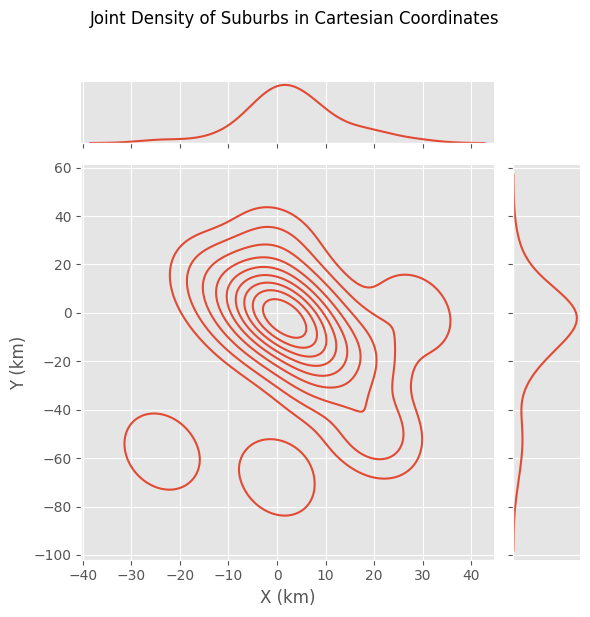
\includegraphics[scale=0.5]{figures/joint_density.png}
      \label{fig:jd_suburb_dist}
  }
  \hspace{0cm} % Adjust horizontal spacing
  \subfigure[Scatterplot of the Suburbs]{
      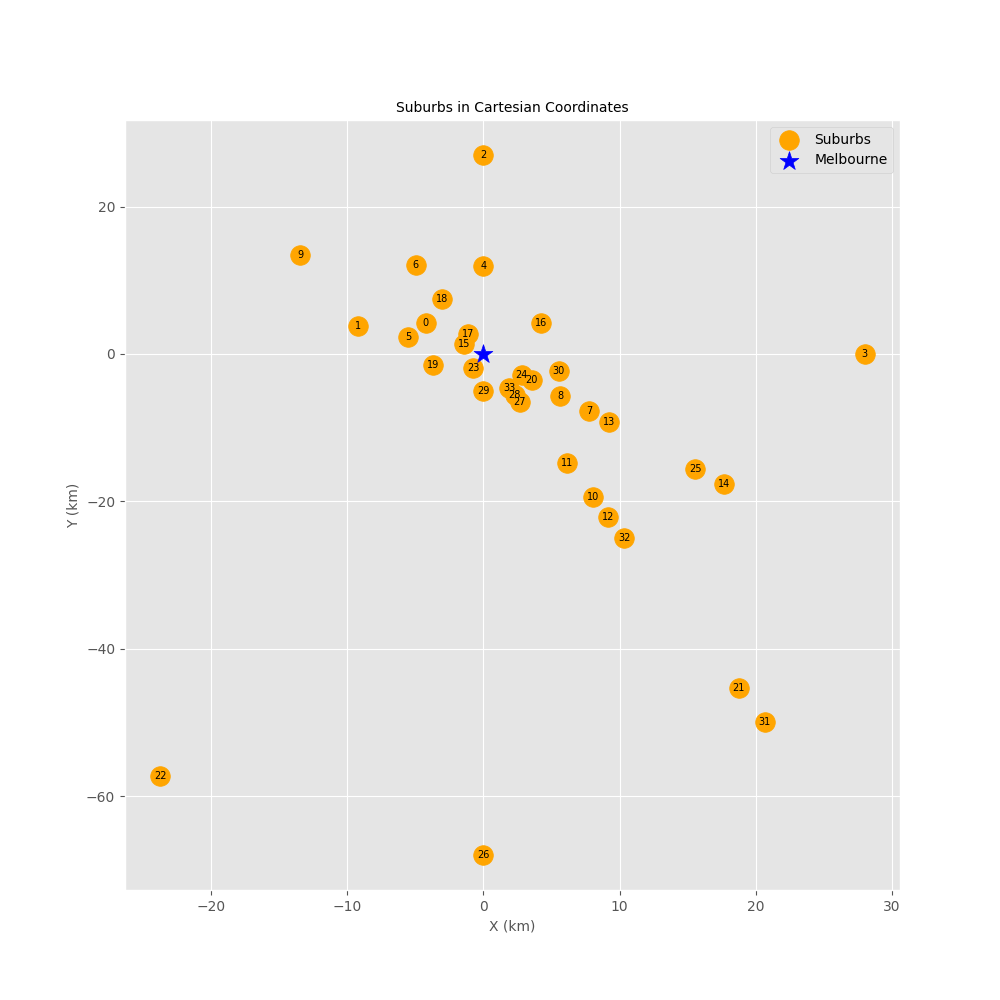
\includegraphics[scale=0.3]{suburbs_cartesian.png}
      \label{fig:scatter_suburb}
  }
  
  \vspace{0cm} % Adjust vertical spacing between rows of figures
  
  \subfigure[MDS of Services]{
      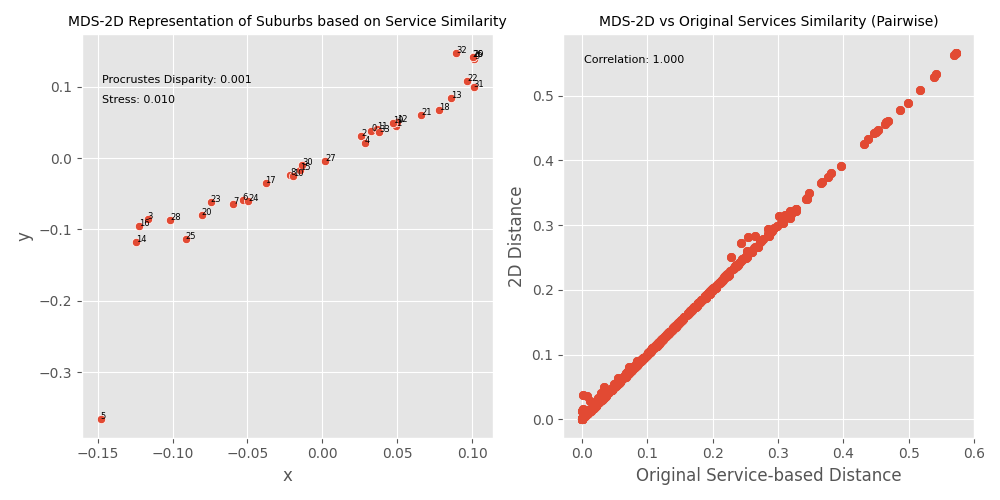
\includegraphics[scale=0.5]{mds_services.png}
      \label{fig:mds_services}
  }
  \subfigure[MDS Population Fraction]{
    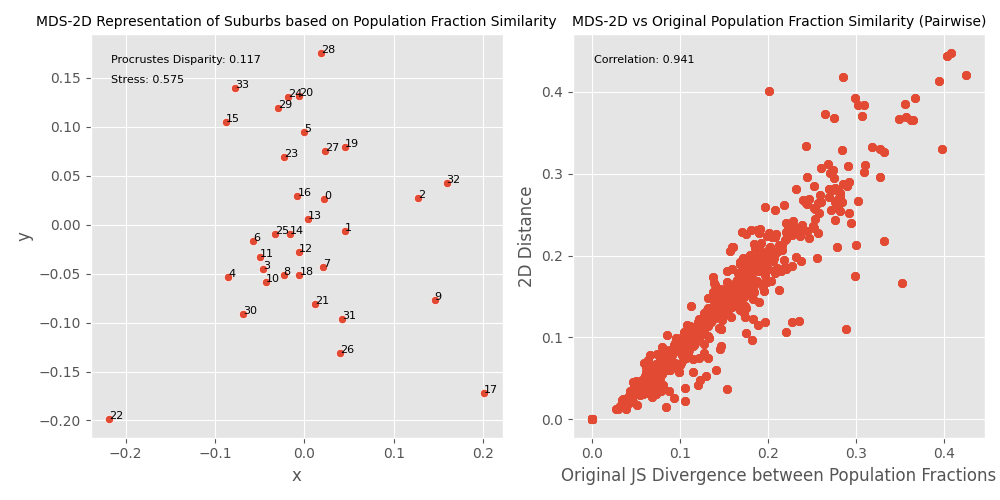
\includegraphics[scale=0.5]{MDS_Population_Fraction.png}
    \label{fig:mds_population}
}
  \hspace{-0.4cm}
  \subfigure[Spectral Clustering]{
      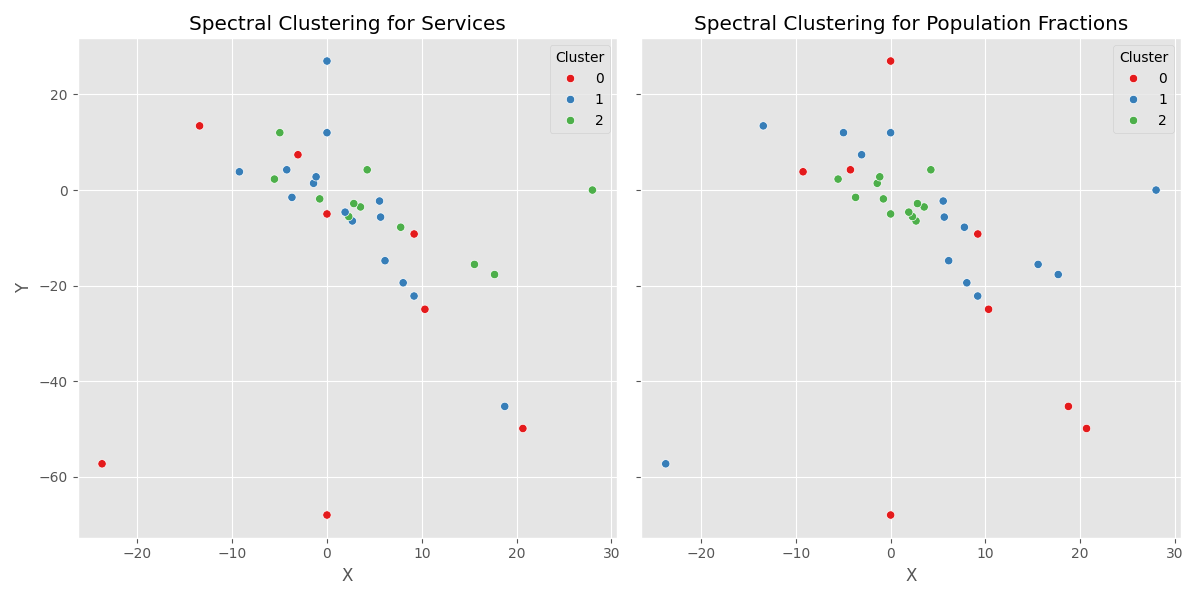
\includegraphics[scale=0.42]{spectral_clustering.png}
      \label{fig:spectral_clustering}
  }
\end{figure}

\begin{figure}
  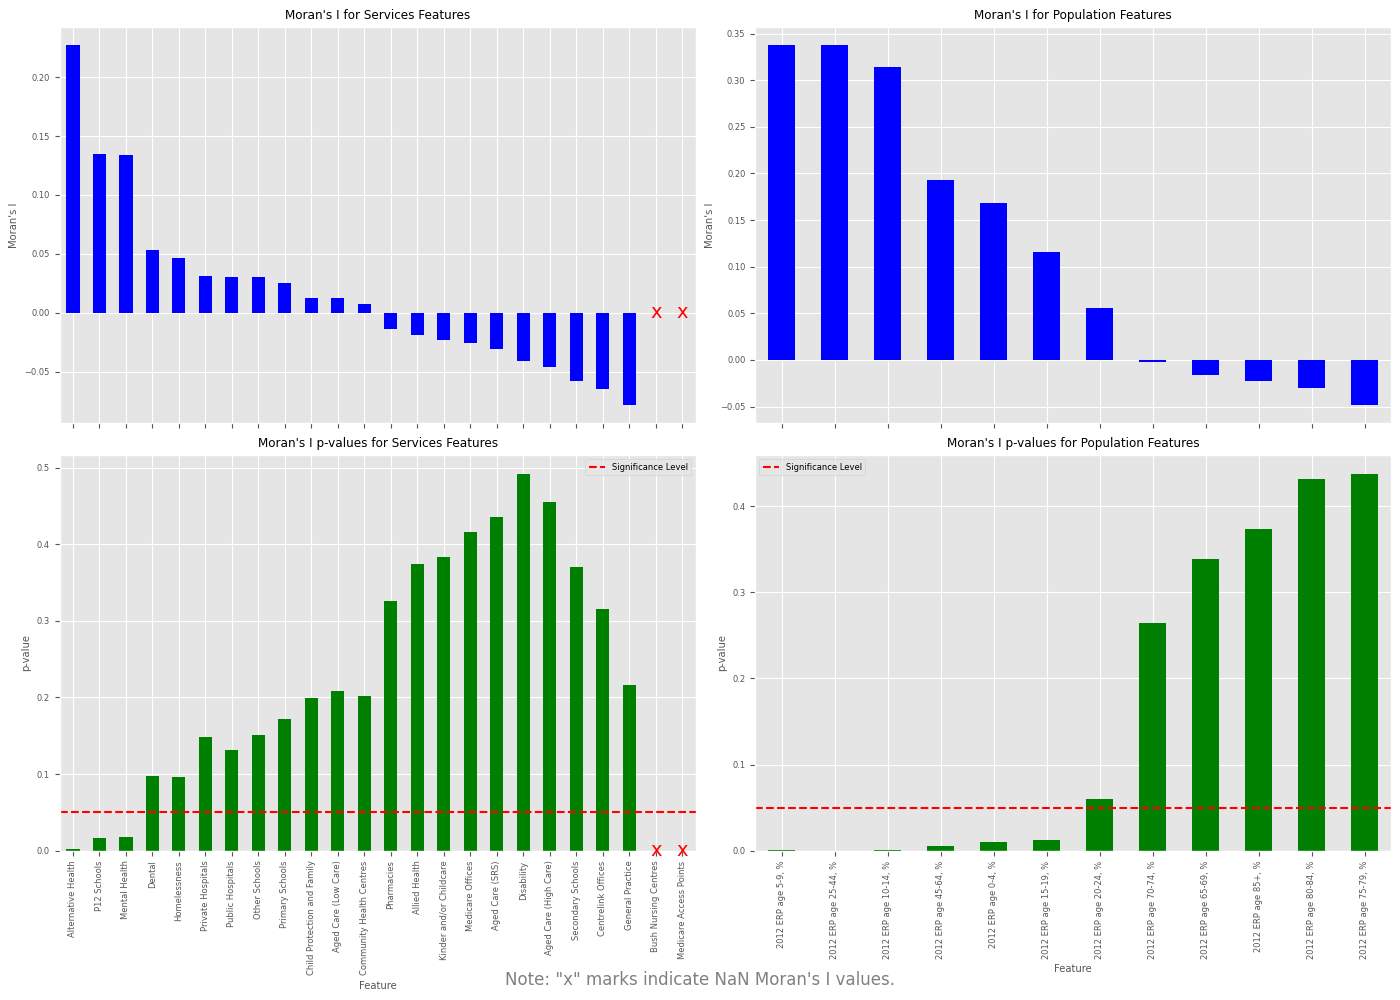
\includegraphics[scale=0.5]{moran_i_analysis.png}
  \caption{Moran's I analysis for the features}
  \label{fig:moran_part_A}
\end{figure}



\pagebreak
\clearpage

\begin{table}[h!]
    \centering
    \begin{tabular}{|c|l|c|l|c|l|}
    \hline
    \textbf{Index} & \textbf{Community Name} & \textbf{Index} & \textbf{Community Name} & \textbf{Index} & \textbf{Community Name} \\ \hline
    0  & Ascot Vale          & 12 & Mordialloc         & 24 & South Yarra         \\
    1  & Braybrook           & 13 & Murrumbeena        & 25 & Springvale          \\
    2  & Craigieburn         & 14 & Noble Park         & 26 & St Andrews Beach    \\
    3  & Croydon             & 15 & North Melbourne    & 27 & St Kilda East       \\
    4  & Fawkner             & 16 & Northcote          & 28 & St Kilda            \\
    5  & Footscray           & 17 & Parkville          & 29 & St Kilda West       \\
    6  & Glenroy             & 18 & Pascoe Vale South  & 30 & Toorak              \\
    7  & Malvern East        & 19 & Port Melbourne     & 31 & Tyabb               \\
    8  & Malvern             & 20 & Prahran            & 32 & Waterways           \\
    9  & Melbourne Airport   & 21 & Somerville         & 33 & Windsor             \\
    10 & Mentone             & 22 & Sorrento           &     &                     \\
    11 & Moorabbin           & 23 & South Melbourne    &     &                     \\
    \hline
    \end{tabular}
    \caption{Index of Communities}
    \label{tab:merged_community_names_serial}
\end{table}

\hspace{-1cm}
\begin{table}[h!]
\fontsize{8}{6}\selectfont % Set font size for the table
\setlength{\tabcolsep}{2pt} % Reduce the space between columns
\renewcommand{\arraystretch}{1.5} % Increase the row height
\begin{tabular}{|p{2cm}|p{2cm}|p{1.5cm}|p{1.5cm}|p{1cm}|p{1cm}|p{1cm}|p{1cm}|p{1cm}|p{1cm}|p{1cm}|p{1cm}|p{1cm}|p{1cm}|} % Add vertical bars between columns with wrapping
\hline
y & X & const & const\_pval & x\_coef & x\_pval & y\_lag & y\_pval & x\_lag & x\_pval & pR\^{}2 & d\_imp & i\_imp & t\_imp \\
\hline
Public hospital separations, 2012-13 & 2012 ERP, total & 369.292 & 0.714 & 0.268 & 0.000 & 0.615 & 0.001 & -0.200 & 0.030 & 0.866 & 0.268 & -0.091 & 0.177 \\
\hline
Population Density & Distance to nearest public hospital & 2176.540 & 0.039 & -242.93 & 0.000 & 0.603 & 0.002 & 7.152 & 0.964 & 0.655 & -242.93 & -351.51 & -594.43 \\
\hline
Category 4 \& 5 emergency department presentations, \% & Distance to nearest public hospital with emergency department & 17.092 & 0.036 & -0.418 & 0.014 & 0.754 & 0.000 & -0.331 & 0.419 & 0.610 & -0.418 & -2.628 & -3.046 \\
\hline
Holds degree or higher, \% & Top occupation, \% & -13.875 & 0.016 & 1.136 & 0.000 & 0.553 & 0.007 & 0.025 & 0.957 & 0.899 & 1.136 & 1.461 & 2.597 \\
\hline
Equivalent household income \$600/week, \% & Dwellings with no internet, \% & 2.979 & 0.641 & 1.392 & 0.000 & 0.638 & 0.000 & -0.682 & 0.201 & 0.729 & 1.392 & 0.570 & 1.962 \\
\hline
\end{tabular}
\caption{Summary of SDMs}
\label{tab:summary_SDM}
\end{table}


\begin{small}
  y: Dependent Variable, X: Predictor Variable, const: Constant Coefficient, const\_pval: Constant p-value, x\_coef: Predictor Coefficient, x\_pval: Predictor p-value, y\_lag: Dependent Variable Lag, y\_pval: p-value for Dependent Lag, x\_lag: Predictor Variable Lag, x\_pval: p-value for Predictor Lag, pR\^{}2: Pseudo R-squared, d\_imp: Direct Impact, i\_imp: Indirect Impact, t\_imp: Total Impact.
\end{small}


\twocolumn
\printbibliography

\end{document}